%-----------------------circuit 2--------------------------
\section{Single Phase Half Wave Uncontrolled Rectifier with RL load}

\subsection{Circuit used for simulation}

% figure that is centered on the page
\begin{figure}[h]
    \centering
    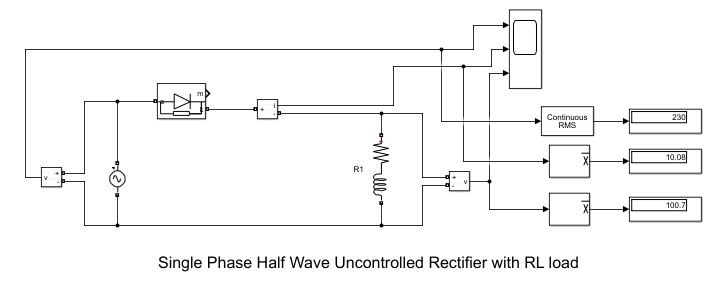
\includegraphics[width=0.7\textwidth]{images/experiment-1/circuit-diagram-simulation-02.png}
    \caption{Circuit used for simulation}
    \label{Fig_simulation_circuit_single-phase-half-wave-uncontrolled-rectifier-with-RL-load}
\end{figure}

\subsection{Components Required}

\begin{table}[h]
    \renewcommand{\arraystretch}{1.3}
    \caption{Components for Single Phase Half Wave Uncontrolled Rectifier with RL load
        load}
    \label{table_components_required_circuit_2}
    \centering
    \begin{tabular}{|c|c|c|c|}
        \hline
        Sr. No & Parameters                     & Ratings            & Quantity \\
        \hline
        \hline
        1      & AC Single Phase Voltage Source & 230V ($ V_{rms} $) & 1        \\
        \hline
        2      & Resistor                       & 10$ \Omega $       & 1        \\
        \hline
        3      & Inductor                       & 10mH               & 1        \\
        \hline
        4      & Diode                          & -                  & 1        \\
        \hline
        5      & Voltmeter                      & -                  & 2        \\
        \hline
        6      & Ammeter                        & -                  & 1        \\
        \hline
    \end{tabular}
\end{table}


\subsection{Resultant Waveforms}

% figure that is centered on the page
\begin{figure}[h]
    \centering
    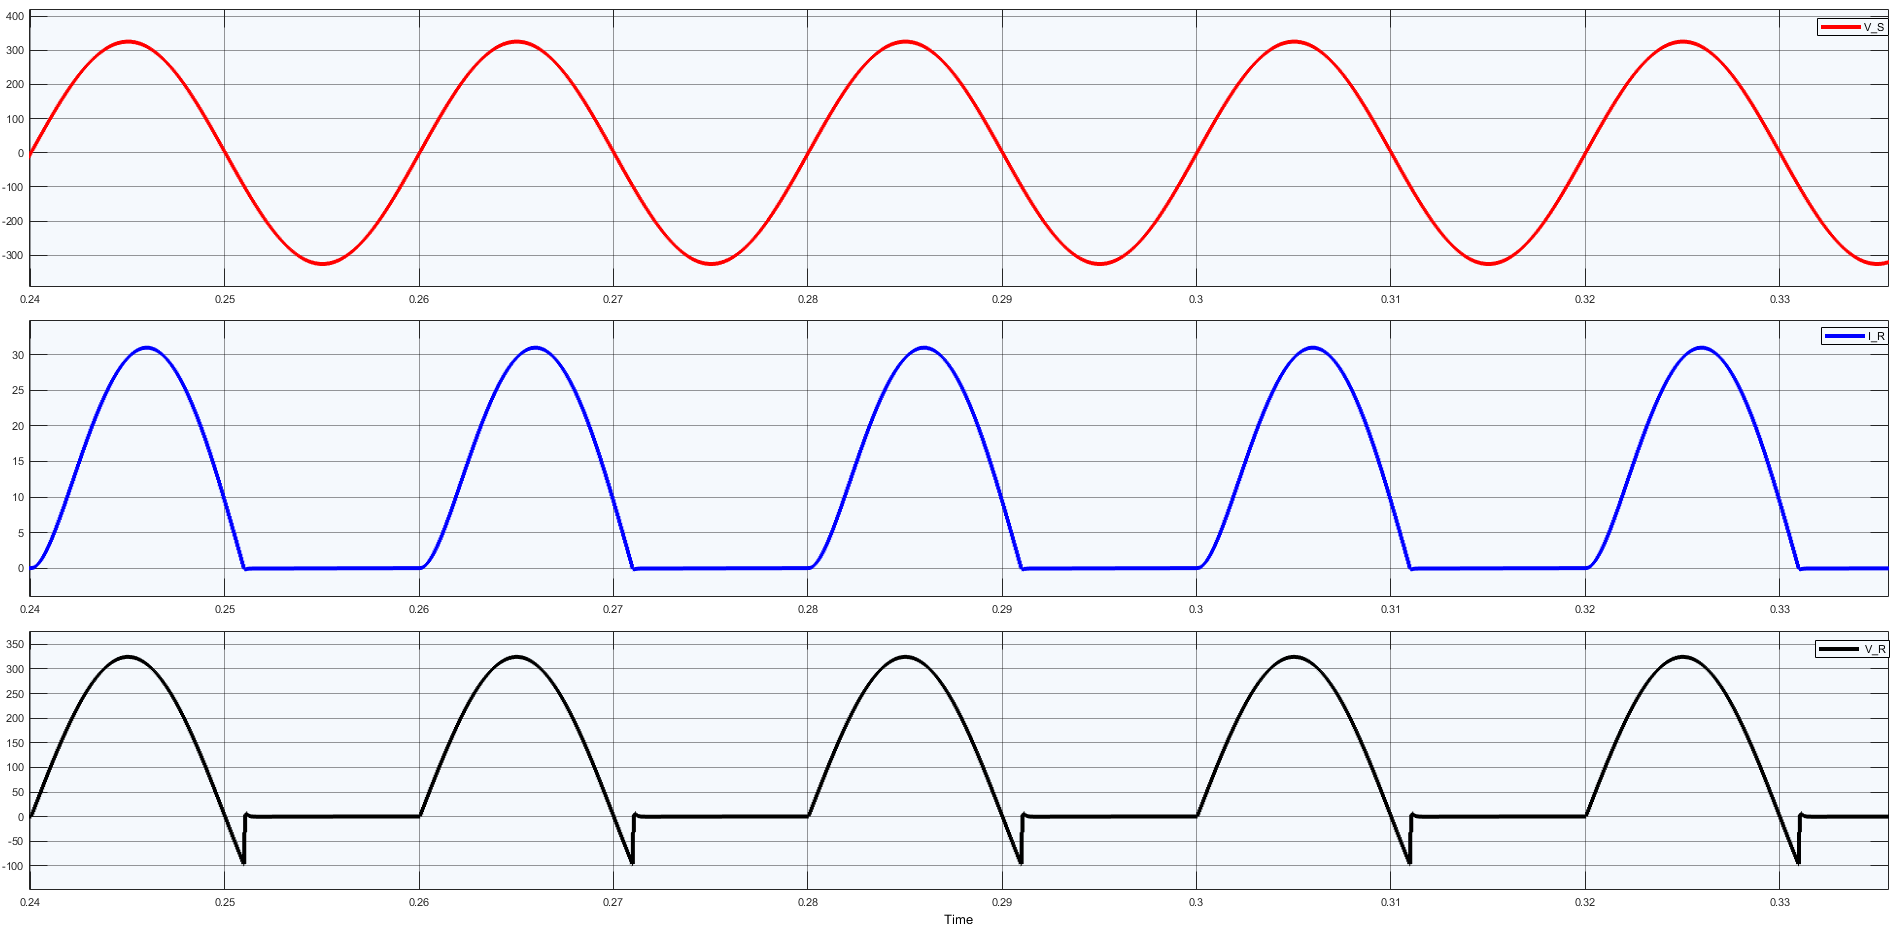
\includegraphics[width=1\textwidth]{images/experiment-1/circuit-scope-simulation-02.png}
    \caption{Circuit used for simulation}
    \label{Fig_waveform_single-phase-half-wave-uncontrolled-rectifier-with-RL-load}
\end{figure}

\subsection{Observations}

\begin{table}[h]
    \renewcommand{\arraystretch}{1.3}
    \caption{Observations for Single Phase Half Wave Uncontrolled Rectifier with R
        load}
    \label{table_observation_2}
    \centering
    \begin{tabular}{|c|c|c|}
        \hline
        Parameters                              & Theoretical Values & Simulation Values \\
        \hline
        \hline
        AC Input Voltage ($ V_{in,rms} $)       & 230V               & 230V              \\
        \hline
        Output Average Voltage ($ V_{o,avg} $)  & 103.53V            & 101.1V            \\
        \hline
        Output Average Current ($ I_{o,avg}  $) & 10.35A             & 10.11A            \\
        \hline
    \end{tabular}
\end{table}


It is observed that the simulated values accurately match the the-
oretical values. As the load is resistive in nature, the output current
is in phase with output voltage. From the output voltage and cur-
rent waveforms, it can be deduced that the diode gets forward biased
during the positive half cycle of the AC source.

